%----------------------------------------------------------------------------------------
%   PACKAGES AND OTHER DOCUMENT CONFIGURATIONS
%----------------------------------------------------------------------------------------

\documentclass[paper=a4, fontsize=11pt]{scrartcl} % A4 paper and 11pt font size
\usepackage{fancyhdr} % Required for custom headers
\usepackage{lastpage} % Required to determine the last page for the footer
\usepackage{extramarks} % Required for headers and footers
\usepackage[usenames,dvipsnames]{color} % Required for custom colors
\usepackage{graphicx} % Required to insert images
\usepackage{listings} % Required for insertion of code
\usepackage{courier} % Required for the courier font
\usepackage{lipsum} % Used for inserting dummy 'Lorem ipsum' text into the template
\usepackage[T1]{fontenc} % Use 8-bit encoding that has 256 glyphs
\usepackage[english]{babel} % English language/hyphenation
\usepackage{amsmath,amsfonts,amsthm} % Math packages

\usepackage{sectsty} % Allows customizing section commands
\allsectionsfont{\centering \normalfont\scshape} % Make all sections centered, the default font and small caps

\pagestyle{fancyplain} % Makes all pages in the document conform to the custom headers and footers
\fancyhead{} % No page header - if you want one, create it in the same way as the footers below
\fancyfoot[L]{} % Empty left footer
\fancyfoot[C]{} % Empty center footer
\fancyfoot[R]{\thepage} % Page numbering for right footer
\renewcommand{\headrulewidth}{0pt} % Remove header underlines
\renewcommand{\footrulewidth}{0pt} % Remove footer underlines
\setlength{\headheight}{13.6pt} % Customize the height of the header

\numberwithin{equation}{section} % Number equations within sections (i.e. 1.1, 1.2, 2.1, 2.2 instead of 1, 2, 3, 4)
\numberwithin{figure}{section} % Number figures within sections (i.e. 1.1, 1.2, 2.1, 2.2 instead of 1, 2, 3, 4)
\numberwithin{table}{section} % Number tables within sections (i.e. 1.1, 1.2, 2.1, 2.2 instead of 1, 2, 3, 4)

\setlength\parindent{0pt} % Removes all indentation from paragraphs - comment this line for an assignment with lots of text

%----------------------------------------------------------------------------------------
%   TITLE SECTION
%----------------------------------------------------------------------------------------

\newcommand{\horrule}[1]{\rule{\linewidth}{#1}} % Create horizontal rule command with 1 argument of height

\title{ 
\normalfont \normalsize 
\textsc{Oregon State University} \\ [25pt]
\horrule{0.5pt} \\[0.4cm] % Thin top horizontal rule
\huge CS 325: Homework 2 \\ % The assignment title
\horrule{2pt} \\[0.5cm] % Thick bottom horizontal rule
}

\author{Colin Bradford} % Your name

\date{\normalsize\today} % Today's date or a custom date

\begin{document}

\maketitle % Print the title

%----------------------------------------------------------------------------------------
%   PROBLEM 1
%----------------------------------------------------------------------------------------
\begin{description}
    \item[1.] \hfill \\
        \begin{description}
        \item[a.] $f(n) = O(g(n))$ \\
            Using a limit results in a simplified expression $\frac{ 10000 }{ 0.00001n - 100 }$. The limit for
            this expression goes to 0 which means that it must be $O(g(n))$.
        \item[b.] $f(n) = \Theta(g(n))$ \\
            Using the limit method, and simplifying using the power rule we get that the limit of the expression
            goes to $10^4$ which is satisifies the limit method rule for $\Theta(g(n))$.
        \item[c.] $f(n) = O(g(n))$ \\
            Using the limit method, the expression can be simplified to $\frac{ 1 }{ n^{0.25} }$ which goes to 0
            and thus must be $O(g(n))$.
        \item[d.] $f(n) = O(g(n))$ \\
            Using the limit method, the expression can be simplified using the l'Hopital's Rule to $\frac{ 1 }{ \ln{10}\log{n} }$
            which goes to 0 and thus must be $O(g(n))$.
        \item[e.] $f(n) = \Omega(g(n))$ \\
            Using the limit method, the expression can be simplified using the l'Hopital's Rule twice to
            $\ln(10)n$ which goes to $\infty$ and thus must be $\Omega(g(n))$.
        \item[f.] $f(n) = O(g(n))$ \\
            Using the limit method, the expression can be simplified using l'Hopital's Rule and some log properties to
            $\frac{ \ln{10} }{ 2\ln{2}\log{3n} }$ which goes to 0 and thus must be $O(g(n))$.
        \item[g.] $f(n) = \Theta(g(n))$ \\
            Using the limit method, the expression can be simplified using log properties to $\log{2}$ which is a constant
            and thus must be $\Theta(g(n))$.
        \item[h.] $f(n) = \Omega(g(n))$ \\
            Using the limit method, if we assume $n = 2^k$ where $k > 0$ and approaches $\infty$, thus we can simplify the expression
            to $\frac{ 2^{2^{k}} }{ 2^{5k} }$ which approaches $\infty$ and thus must be $\Omega(g(n))$.
        \item[i.] $f(n) = \Omega(g(n))$ \\
            Using the limit method, we can replace $2^n = e^{n\ln{2}}$ which allows us to simplify the entire expression to
            $e^{n(1 - \ln{2})}$, since $\ln{2} < 1$ then we can conclude that this limit goes to $\infty$ and thus must be
            $\Omega(g(n))$.
        \item[j.] $f(n) = \Theta(g(n))$ \\
            Using the limit method, the expression can be simplified to $2^n2^{n - 1} = 2^{-1} = \frac{ 1 }{ 2 }$ which is a constant
            and thus must be $\Theta(g(n))$.
        \item[k.] $f(n) = O(g(n))$ \\
            Using the limit method, the expression is trivial as $2^n$ grows much faster than $n$ and thus the limit goes to 0 and as
            a result it must be $O(g(n))$.
        \item[l.] $f(n) = O(g(n))$ \\
            Using the limit method, the expression can be simplified to $n$ which goes to $\infty$ and thus must be $O(g(n))$.
        \item[m.] $f(n) = O(g(n))$ \\
            Using the limit method, we can rewrite the expression as $\frac{2}{1} \cdot \frac{2}{2} \cdot \frac{2}{3} \cdot \ldots \cdot \frac{2}{n}$
            we know that $\frac{2}{n}$ goes to 0 as $n$ goes to $\infty$ and thus we can conclude that the expression approaches 0 as $n$
            approaches $\infty$ and finally that means that it must be $O(g(n))$.
        \item[n.] $f(n) = \Omega(g(n))$ \\
            Using the limit method, the expression can be simplified to $n + 1$ which goes to $\infty$ and thus must be $\Omega(g(n))$.
        \end{description}
    \item[2.] \hfill \\
        \begin{description}
        \item[a.] \hfill \\
            Assume $f_1(n) = O(f_2(n))$ and $f_2(n) = O(f_1(n))$ \\
            Since we know that $\lim_{n \to \infty} \frac{ f_1(n) }{ f_2(n) } = 0$ \\
            Then $\lim_{n \to \infty} \frac{ f_2(n) }{ f_1(n) } = \infty$ must be true \\
            However, this contradicts our assumption of $f_2(n) = O(f_1(n))$ which would require $\lim_{n \to \infty} \frac{ f_2(n) }{ f_1(n) } = 0$ \\
            Thus, if $f_1(n) = O(f_2(n))$ then $f_2(n) = O(f_1(n))$ cannot be true.
        \item[b.] \hfill \\
            Assume $f_1(n) = O(g_1(n))$ and $f_2(n) = O(g_2(n))$, then $f_1(n) \cdot f_2(n) = O(g_1(n) \cdot g_2(n))$. \\
            By definition $f_1(n) \leq c_1g_1(n)$ and $f_2(n) \leq c_2g_2(n)$ \\
            Thus we can say $f_1(n) \cdot f_2(n) \leq c_1c_2g_1(n) \cdot g_2(n)$ \\
            We can rewrite it as $f_1(n) \cdot f_2(n) \leq c_3g_1(n) \cdot g_2(n)$ \\
            Thus we have proven the statement true.
        \item[c.] \hfill \\
            Assume $\max{(f_1(n), f_2(n))} = \Theta(f_1(n) + f_2(n))$ \\
            By definition $c_1(f_1(n) + f_2(n)) \leq \max{(f_1(n), f_2(n))} \leq c_2(f_1(n) + f_2(n))$ \\
            By definition $\max{(f_1(n), f_2(n))} \leq f_1(n) + f_2(n)$, thus $c_2 = 1$ \\
            By definition there is some $c_{f1}$ for $f_1(n)$ and some $c_{f2}$ for $f_2(n)$ \\
            We only care about the largest $c$ so we can say that $c_1 = \max{(c_{f1}, c_{f2})}$ \\
            Thus we have proven the afformentioned statement.
        \end{description}
    \item[3.] \hfill \\
        \begin{description}
        \item[a.] \hfill \\
            Prove $F_n \geq 2^{0.5n}$ for $n \geq 6$ \\
            Given $F_n = F_{n - 1} + F_{n - 2}$ \\
            and $F_0 = 0$ \\
            and $F_1 = 1$ \\
            and $F_6 = 8$ \\
            and $F_7 = 13$ \\
            \begin{description}
            \item[Base case n = 6] \hfill \\
            \begin{align}
            \begin{split}
                F_n & \geq 2^{0.5n} \\
                F_6 & \geq 2^3 \\
                8 & \geq 8 \\
                F_n & \geq 2^{0.5n} \\
                F_7 & \geq 2^{3.5} \\
                13 & \geq 8
            \end{split}
            \end{align}
            The inequality holds true for the base case of $n = 6$
            \item[Inductive case] \hfill \\
            Assume $F_{n + 1} = F_n + F_{n - 1}$ \\
            and $F_n \geq 2^{0.5n}$ and $F_{n - 1} \geq 2^{0.5(n - 1)}$ for all $n \geq 8$ \\
            \begin{align}
            \begin{split}
                F_{n + 1} & \geq 2^{0.5(n + 1)} \\
                F_n + F_{n - 1} & \geq 2^{0.5(n + 1)} \\
                2^{0.5n} + 2^{0.5(n + 1)} & \geq 2^{0.5(n + 1)} \\
                2^{0.5n} + 2^{0.5n}2^{-0.5} & \geq 2^{0.5n}2^{0.5} \\
                1 + 2^{-0.5} & \geq 2^{0.5} \\
                1.707 & \geq 1.414
            \end{split}
            \end{align}
            The inequality holds true, thus $F_n \geq 2^{0.5n}$ for $n \geq 6$ has been proven.
            \end{description}
        \item[b.] \hfill \\
            Using the same principle used in part a, as long as the inequality $2^{cn} + 2^{c(n + 1)} \leq 2^{c(n + 1)}$ holds true 
            $n \geq 0$, the $c$ is correct. \\
            Let $c = 0.9$ \\
            \begin{align}
            \begin{split}
                2^{0.9n} + 2^{0.9(n - 1)} & \leq 2^{0.9(n + 1)} \\
                2^{0.9n} + 2^{0.9n}2^{-0.9} & \leq 2^{0.9n}2^{0.9} \\
                1 + 2^{-0.9} & \leq 2^{0.9} \\
                1.535 & \leq 1.866
            \end{split}
            \end{align}
            The inequality holds true and thus $0.9$ is an acceptable value for $c$.
        \item[c.] \hfill \\
            \begin{align}
            \begin{split}
                F_{n} & \leq 2^{c(n + 1)} \\
                2^{c(n - 1)} + 2^{c(n - 2)} & \leq 2^{c(n)} \\
                2^{cn}2^{-c} + 2^{cn}2^{-2c} & \leq 2^{c(n)} \\
                2^{-c} + 2^{-2c} & \leq 1 \\
            \end{split}
            \end{align}
            Substitute $x$ for $2^{-c}$
            \begin{align}
            \begin{split}
                x + x^2 & \leq 1 \\
                x^2 + x - 1 & \leq 0 \\
            \end{split}
            \end{align}
            We can solve for $x$ and then for $c$ which leaves us with $\phi$ (the golden ratio) \\
            Thus, the largest $c$ we can find is when $c = \phi$.
        \end{description}
    \item[4.] \hfill \\
        $\phi = \frac{ 1 + \sqrt{5} }{ 2 }$ \\
        \begin{align}
        \begin{split}
            x^2 - x - 1 & = 0 \\
            (\frac{ 1 + \sqrt{5} }{ 2 })^2 - (\frac{ 1 + \sqrt{5} }{ 2 }) - 1 & = 0 \\
            \frac{ 1 + 2\sqrt{5} + 5 }{ 4 } - (\frac{ 1 + \sqrt{5} }{ 2 }) - 1 & = 0 \\
            \frac{ 1 + 2\sqrt{5} + 5 }{ 4 } - (\frac{ 2 + 2\sqrt{5} }{ 4 }) - \frac{ 4 }{ 4 } & = 0 \\
            1 + 2\sqrt{5} + 5 - 2 - 2\sqrt{5} - 4 & = 0 \\
            6 - 6 + 2\sqrt{5} - 2\sqrt{5} & = 0 \\
            0 &= 0
        \end{split}
        \end{align}
        $\Phi = \frac{ 1 - \sqrt{5} }{ 2 }$ \\
        \begin{align}
        \begin{split}
            x^2 - x - 1 & = 0 \\
            (\frac{ 1 - \sqrt{5} }{ 2 })^2 - (\frac{ 1 - \sqrt{5} }{ 2 }) - 1 & = 0 \\
            \frac{ 6 - 2\sqrt{5} }{ 4 } - (\frac{ 1 - \sqrt{5} }{ 2 }) - 1 & = 0 \\
            \frac{ 6 - 2\sqrt{5} }{ 4 } - (\frac{ 2 - 2\sqrt{5} }{ 4 }) - \frac{ 4 }{ 4 } & = 0 \\
            6 - 2\sqrt{5} - 2 + 2\sqrt{5} - 4 & = 0 \\
            6 - 6 + 2\sqrt{5} - 2\sqrt{5} & = 0 \\
            0 &= 0
        \end{split}
        \end{align}
    \item[5.] \hfill \\
        \begin{description}
        \item[a.] Implementation \\
    \begin{lstlisting}[language=Python]
    # Written in Python
    import time

    def main():
        test_vals = [ 4, 8, 10, 16, 20, 25 ]
        bc_one_vals = []
        bc_two_vals = []
        for test_val in test_vals:
            n = test_val
            k = n / 2
            # test bc_one
            start_time = time.time()
            bc_one(n, k)
            bc_one_vals.append((n, time.time() - start_time))
            # test bc_two
            start_time = time.time()
            bc_two(n, k)
            bc_two_vals.append((n, time.time() - start_time))
        for val in bc_one_vals:
            print("[BC1] %u: %s s" % val)
        for val in bc_two_vals:
            print("[BC2] %u: %s s" % val)
    
    def bc_one(n, k):
        if (k == n or k == 0):
            return 1
        return bc_one(n - 1, k) + bc_one(n - 1, k - 1)
    
    def bc_two(n, k):
        if (k == 0):
            return 1
        return bc_two(n - 1, k - 1) * (n / k)
    
    if __name__ == '__main__':
        main()
    \end{lstlisting}


    \item[b.] Below are the running times \\
    \begin{lstlisting}
    Algorithm |  n | time (seconds)
              |    |
    [BC1]     |  4 | 5.96046447754e-06 s
    [BC1]     |  8 | 3.50475311279e-05 s
    [BC1]     | 10 | 0.000120878219604 s
    [BC1]     | 16 | 0.00579380989075 s
    [BC1]     | 20 | 0.0890920162201 s
    [BC1]     | 25 | 2.44316911697 s
              |    |
    [BC2]     |  4 | 1.90734863281e-06 s
    [BC2]     |  8 | 2.14576721191e-06 s
    [BC2]     | 10 | 2.14576721191e-06 s
    [BC2]     | 16 | 3.09944152832e-06 s
    [BC2]     | 20 | 5.00679016113e-06 s
    [BC2]     | 25 | 6.91413879395e-06 s
    \end{lstlisting}

    \item[c.] Graph \\
    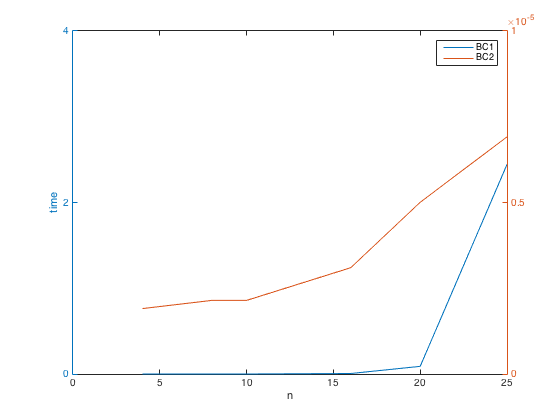
\includegraphics[width=\textwidth]{hw2Fig}
    \end{description}
\end{description}

%----------------------------------------------------------------------------------------

\end{document}